%!TEX root = ../thesis.tex
%*******************************************************************************
%****************************** Third Chapter **********************************
%*******************************************************************************
\chapter{Requirements Elicitation}
\graphicspath{{Chapter4/Figs/Raster/}{Chapter4/Figs/}}

Background literature review in Chapter 2.1 and 2.2 has driven the direction of the project and
provided many ideas for functional requirements. This chapter describes the further collection of primary
data, and provides the list of formal user requirements.

\section{Primary Data and Analysis}
Collecting primary data from shareholders of higher education e-learning systems would be able to:
\begin{itemize}
	\setlength\itemsep{0em}	
	\item reaffirm and further develop requirements obtained from literature in Chapter 2
	\item obtain further requirements from real-world participants, their pain points and goals
\end{itemize}

\subsection{Methodology}

A qualitative study was conducted with semi-structured, face-to-face interviews (open-ended questions). 
The participants were gathered through direct email contact (convenience sampling). 
They were:
\begin{itemize}
	\setlength\itemsep{0em}	
	\item Teaching staff in higher education with 10+ years of experience, and
	\item Students in higher education who has academic liaison experience and are exposed to a wide range of student problems.
\end{itemize}

It was important that a qualitative, semi-structured method is used. 
This allowed for a flexible scope, encouraging the generation of new perspectives and 
ideas beyond that of the secondary research in Chapter 2.
It also increased validity, as the interviewer can probe for a deeper understanding
\citep{mcleod2014interviews}.

An ethics submission was completed on BREO and approval was granted on 21st November.
See Supporting Materials/Ethics/Requirements/ for the approved 
participant information sheet, consent form and example questions documents.

A total of five interviews were conducted between December 2017 and February 2018:
two with teaching staff and three with student representatives. See table
\ref{table:participants-req} for a more detailed description of these participants.

\begin{table}[!h]
	\caption{Participants in primary data collection interviews}
	\centering
	\label{table:participants-req}
	\begin{tabularx}{\textwidth}{>{\bfseries}lX}
		Participant & Characterisation                                                                    \\
		\toprule
		Educator A  & lecturer in higher education for over 20 years, and an experienced higher education
		administrator                                                                                     \\\midrule
		Educator B  & lecturer in higher education for over 20 years, with research interests
		in e-learning interactions, effectiveness and acceptance                                          \\\midrule
		Student C   & a university course representative for 3 years, which involves collecting and
		communicating student feedback and attending staff-student liaison meetings                       \\\midrule
		Student D   & a university peer-assisted learning leader for 2 years, helping out lower level
		students with their academic work by facilitating peer discussions, and escalating common problems
		to academic staff in debrief sessions                                                             \\\midrule
		Student E   & a university course representative for 2 years and a peer-assisted learning leader
		for 1 year                                                                                        \\\bottomrule
	\end{tabularx}
\end{table}

\subsection{Interview Results and Analysis}

The raw data from interviews (transcripts) were contextually analysed and grouped thematically 
using thematic analysis techniques from \citet{clarke2014thematic}.
These are presented below as problem statements (PS).
These problem statements were sorted into four affinity groups: statements about assessments,
curriculum personalisation, higher education, and e-Learning systems.
 
Below you will find the sample questions asked for each group,
the problem statements, explanations and discussions.
For the relevant transcript snippets for each problem statements, please go to Appendix C.

\subsubsection{On Assessments}

Leading Question: What are the problems with assessments in higher education today? /
Is there tension between students and teachers over assessments, and why?

\begin{table}[!ht]
	\begin{tabularx}{\textwidth}{|c|X|c|}
		\hline
		    & Problem Statement                                      & Participants \\
		\hline
		PS1 & \textbf{Poor communication of assessment expectations} & B, C, D, E   \\
		\hline
		\multicolumn{3}{|X|}{Four participants have independently confirmed that the problem with transparency in expectations for
			assessments (as described in Chapter 2.1.1) does exist.}                    \\
		\hline
	\end{tabularx}
\end{table}
\begin{table}[!ht]
	\begin{tabularx}{\textwidth}{|c|X|c|}
		\hline
		PS2 & \textbf{Lack of practice and formative feedback} & B, D       \\
		\hline
		\multicolumn{3}{|X|}{Students transitioning from school to higher education would experience a drop in formative assessments
			(that do not affect their final grade) such as homework practices.} \\
		\hline
	\end{tabularx}
\end{table}
\begin{table}[!ht]
	\begin{tabularx}{\textwidth}{|c|X|c|}
		\hline
		PS3 & \textbf{Lack of standardisation in marking criteria} & B, C, E \\
		\hline
		\multicolumn{3}{|X|}{Some assessments have clearly defined marking criteria forms for markers, but a high
			number of them do not.}                                              \\
		\hline
	\end{tabularx}
\end{table}
\begin{table}[!ht]
	\begin{tabularx}{\textwidth}{|c|X|c|}
		\hline
		PS4 & \textbf{Oral defence may be necessary to validate assessments} & A, E                 \\
		\hline
		\multicolumn{3}{|X|}{Concern was raised over the ease of cheating and incomplete
			learning, especially in automatic assessments. Vivas are proposed as a potential solution.} \\
		\hline
	\end{tabularx}
\end{table}
\begin{table}[!ht]
	\begin{tabularx}{\textwidth}{|c|X|c|}
		\hline
		PS5 & \textbf{Lack of feedback and procedural transparency in terminal assessments} & C \\
		\hline
		\multicolumn{3}{|X|}{Students are unhappy with the lack of, or scarcity of feedback
			from terminal assessments and exams.}                                                   \\
		\hline
	\end{tabularx}
\end{table}
\begin{table}[!ht]
	\begin{tabularx}{\textwidth}{|c|X|c|}
		\hline
		PS6 & \textbf{The need for synoptic (cross-topics) assessments} & B \\
		\hline
		\multicolumn{3}{|X|}{There is a concern that assessments are too
			compartmentalised into their modules, not relevant to industry and not encouraging
			holistic critical thinking.}                                       \\
		\hline
	\end{tabularx}
\end{table}

The interviews have confirmed the problem of transparency on assessments (see PS1, PS3, PS5), 
while new user concerns have surfaced, namely the lack of practice (PS2), the need 
for assessment validations (PS4), and synoptic assessments (PS6).

Most of these problems can be tackled by a blockchain-based system. 
The lack of formative feedback (PS2) however, is seen more as a human factor, 
as it depends heavily on how the module is designed by its teacher. 
Synoptic assessments (PS6) are considered a low priority feature, 
as it is a relatively new concept in higher education, and was only mentioned by 
one participant.

\subsubsection{On Curriculum Personalisation}

Leading Question: What do you think are the current roadblocks to offering more multi-disciplinary,
personalised, or even multi-institutional arrangements for higher education?

\begin{table}[!ht]
	\begin{tabularx}{\textwidth}{|c|X|c|}
		\hline
		PS7                                        & \textbf{There is a demand for multi-disciplinary degree offerings but only a few
		universities are capable of offering them} & B, C, D                                                                          \\
		\hline
		\multicolumn{3}{|X|}{A defined degree that encompasses two particular fields may not be economically viable;
			universities struggle with bureaucracy for curriculum personalisation;
			students like more freedom and sometimes dislike certain compulsory modules.}                                                 \\
		\hline
	\end{tabularx}
\end{table}
\begin{table}[!ht]
	\begin{tabularx}{\textwidth}{|c|X|c|}
		\hline
		PS8 & \textbf{Dedicated support and guidance is necessary for increased customisation} & B, E \\
		\hline
		\multicolumn{3}{|X|}{There are careers that require multi-disciplinary backgrounds, but there is a risk of
			students not making informed choices.}                                                        \\
		\hline
	\end{tabularx}
\end{table}
\begin{table}[!ht]
	\begin{tabularx}{\textwidth}{|c|X|c|}
		\hline
		PS9 & \textbf{National regulations requiring programme outcomes and specifications deter movement} & A \\
		\hline
		\multicolumn{3}{|X|}{The UK higher education academic infrastructure requires all degree programme to lay out
			programme outcomes and programme specifications, which deters movement.}                               \\
		\hline
	\end{tabularx}
\end{table}
\begin{table}[!ht]
	\begin{tabularx}{\textwidth}{|c|X|c|}
		\hline
		PS10 & \textbf{Managing study load for multi-disciplinary courses may be difficult} & E \\
		\hline
		\multicolumn{3}{|X|}{Switching between the mindsets for different disciplines could be hard.
			The number of credits for multi-disciplinary programs should not be higher.}            \\
		\hline
	\end{tabularx}
\end{table}

It was encouraging to see that three out of four participants described a clear demand 
for more freedom in curriculum personalisation (PS7). Also confirming the need for 
informed educational decisions as described by \citet{green2005futurelab}, participants 
have asked for dedicated curriculum personalisation support (PS8).

The present inflexible degree structures in markets such as the UK is an interesting 
point raised by participant A (PS9). This is actually what Smart Contracts 
can be very good at, automating manual, regulatory work. For this proof-of-concept 
project, example administrative fields can be added to showcase such potential.

\subsubsection{Other Higher Education Issues}

Leading Question: What else needs improving in higher education in general?

\begin{table}[!ht]
	\begin{tabularx}{\textwidth}{|c|X|c|}
		\hline
		PS11 & \textbf{More support, interaction and engagement needed} & D, E       \\
		\hline
		\multicolumn{3}{|X|}{Students have complained that institutions are not always 
		good at supporting and engaging with all students.} \\
		\hline
	\end{tabularx}
\end{table}
\begin{table}[!ht]
	\begin{tabularx}{\textwidth}{|c|X|c|}
		\hline
		PS12 & \textbf{Administrative middlemen causing delays and bottlenecks in institutions} & E                \\
		\hline
		\multicolumn{3}{|X|}{Students complained that feedback was not given on time due to administrative delays} \\
		\hline
	\end{tabularx}
\end{table}
\begin{table}[!ht]
	\begin{tabularx}{\textwidth}{|c|X|c|}
		\hline
		PS13 & \textbf{Lack of support on self-regulated learning skills} & B                                                      \\
		\hline
		\multicolumn{3}{|X|}{There is not enough help and guidance for students to make the transition to self-motivated learning} \\
		\hline
	\end{tabularx}
\end{table}

Only the administrative bottleneck issue (PS12) is considered highly relevant to this project. 
A blockchain backend would not be able to improve student engagement (PS11) or self-regulated learning skills (PS13).

\subsubsection{e-Learning System Issues}

Sample Questions: What other features would you like to see in a future e-Learning system for
higher education?

\begin{table}[!ht]
	\begin{tabularx}{\textwidth}{|c|X|c|}
		\hline
		PS14 & \textbf{Fine-grained access control for learning history needed to preserve privacy} & D, E \\
		\hline
		\multicolumn{3}{|X|}{Students prefer to be as private as possible, and dislike data aggregation, 
		even by their institution}  \\
		\hline
	\end{tabularx}
\end{table}
\begin{table}[!ht]
	\begin{tabularx}{\textwidth}{|c|X|c|}
		\hline
		PS15 & \textbf{Poor mobile friendliness in many e-Learning systems} & C                        \\
		\hline
		\multicolumn{3}{|X|}{Students want any new system to be built responsive and mobile friendly.} \\
		\hline
	\end{tabularx}
\end{table}
\begin{table}[!ht]
	\begin{tabularx}{\textwidth}{|c|X|c|}
		\hline
		PS16 & \textbf{Real-world learning activities not captured in course management systems} & A               \\
		\hline
		\multicolumn{3}{|X|}{For example, face-to-face contact time is not captured by most conventional systems.} \\
		\hline
	\end{tabularx}
\end{table}
\begin{table}[!ht]
	\begin{tabularx}{\textwidth}{|c|X|c|}
		\hline
		PS17 & \textbf{Systems cannot be customised to fit assessment and grading models} & A                              \\
		\hline
		\multicolumn{3}{|X|}{assessment features and functions on e-learning systems are incompatible
			with institutional requirements, or even national requirements, giving staff extra work converting them manually.} \\
		\hline
	\end{tabularx}
\end{table}
\begin{table}[!ht]
	\begin{tabularx}{\textwidth}{|c|X|c|}
		\hline
		PS18 & \textbf{Multiple systems used in concoction without login integration} & B                                 \\
		\hline
		\multicolumn{3}{|X|}{No single sign-on for intranet, assessment, content management and student records systems.} \\
		\hline
	\end{tabularx}
\end{table}
\begin{table}[!ht]
	\begin{tabularx}{\textwidth}{|c|X|c|}
		\hline
		PS19 & \textbf{Lower trust and value associated with online institutions and programmes} & C                \\
		\hline
		\multicolumn{3}{|X|}{It is hard to bridge the gap in trust and reputation that comes with campus learning.} \\
		\hline
	\end{tabularx}
\end{table}

Ease of use is a major theme in this group, with requests for mobile friendliness (PS15), 
flexibility in record types (PS16, 17), and single sign-on (PS18). It will be important 
to take these into account while designing our blockchain and client applications.

A blockchain could also be the technology fit to improve access control (PS14) and 
create trust (PS19). These two user concerns discovered has been added to the objectives 
of the project.

\subsubsection{Summary}

Overall, the study has been useful in extending our knowledge on e-Learning issues.
The convenience sampling has likely been a limitation, since all participants were 
recruited from the same university, and the social circle of the interviewer.

An affinity diagram is also produced to give a high-level overview of all the problem statements.
(See Figure \ref{fig:ps-affinity} on the next page).

\clearpage
\begin{figure}[!ht]
	\centering
	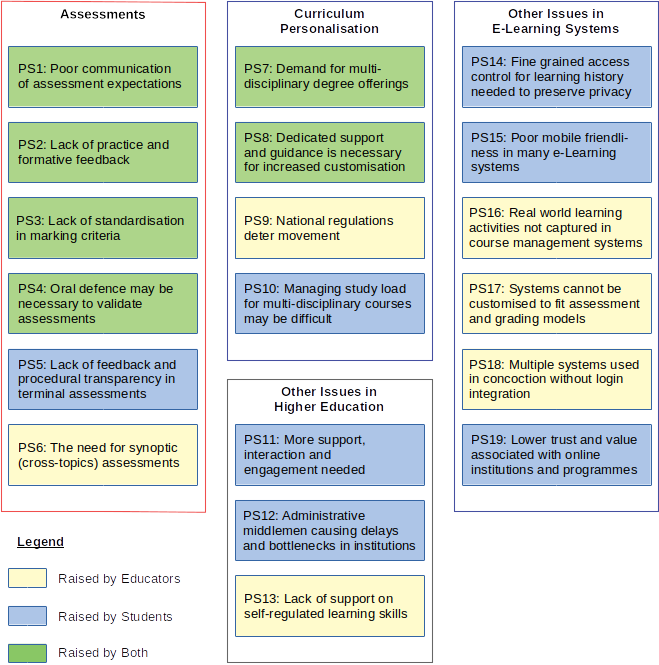
\includegraphics[width=1.0\textwidth]{ps-affinity}
	\caption[Affinity diagram for primary data]
	{Affinity diagram for problem statements devised from primary data}
	\label{fig:ps-affinity}
\end{figure}

\section{Formal Requirements}

Table \ref{table:fx-reqs} lists the functional requirements (FR) adopted by this
project going forward. They are related to one or more of the problem statements (PS) gathered
above from primary data, or to the literature reviewed in Chapter 2.

Table \ref{table:nonfx-reqs} lists the non-functional requirements (NR) adopted by this
project going forward. They are related to one or more of the problem statements (PS) gathered,
or to usability heuristics.

These requirements have been ranked with the MoSCoW prioritisation
framework, which specified four levels of priority: Must Have, Should Have, Could Have, and Won’t Have
this time \citep{agile2018moscow}. The MoSCoW levels are given from mainly a system engineering perspective
in planning the minimum viable product for the demonstrator of this project,
and do not necessarily reflect the priorities of the stakeholders.

\begin{table}[!h]
	\caption{Prioritised list of functional requirements for this project}
	\centering
	\label{table:fx-reqs}
	\begin{tabularx}{\textwidth}{>{\bfseries}l>{\hsize=1.5\hsize}X>{\hsize=.5\hsize}Xl}
		                                                          & Requirement Statements                                                            & Related To  & MoSCoW \\
		\toprule
		FR1                                                       & The system would store learner records on a blockchain
		                                                          & Ch 2.2.1 (LTSA)                                                                   & Must Have
		\\\midrule
		FR2                                                       & Teachers would be able to create and edit learning resources
		                                                          & Ch 2.2.1 (LTSA)                                                                   & Must Have
		\\\midrule
		FR3                                                       & Teachers would be able to create and edit assessments
		                                                          & Ch 2.2.1 (LTSA)                                                                   & Must Have
		\\\midrule
		FR4                                                       & The system would enforce the provision of learning outcomes, knowledge required
		and assessment goals & Ch 2.1.1 (Transparency),
		PS1                                                       & Must Have
		\\\midrule
		FR5                                                       & The system would enforce predefined assessments rules (eg. marking schemes,
		transparent procedures and feedback) with Smart Contracts
		                                                          & Ch 2.1.1 (Transparency), PS3, PS5                                                 & Must Have
		\\\midrule
		FR6                                                       & The system would allow teachers to configure multiple assessments and
		formative assessments for modules                         & PS2                                                                               & Could Have
		\\\midrule
		FR7                                                       & The system would be able to facilitate vivas (oral defence) as a form of assessments         &
		PS4                                                       & Could Have
		\\\midrule
		FR8                                                       & The system would provide multiple ways to define grade schema                     & PS17
		                                                          & Could Have
		\\\midrule
		FR9                                                       & Teachers would be able to negotiate a customised list of courses for a student
		within a fixed course credits budget, customising degree specifications
		                                                          & Ch 2.1.2 (Personalisation), PS7, PS9, PS10                                              & Must Have
		\\\midrule
		FR10                                                      & The system should feature dedicated support channels between students and teachers
		or other advisors
		                                                          & PS8, PS11                                                                         & Should Have
		\\\midrule
		FR11                                                      & Students would be able to add assessment submissions on the blockchain
		                                                          & Figure \ref{fig:moocon_assess} (Concept)                                          & Must Have
		\\\midrule
		FR12                                                      & The system would be able to generate certificates on the blockchain when a course
		has been completed                                        & Figure \ref{fig:moocon_assess} (Concept)                                          & Must Have
		\\\midrule
		FR13                                                      & The system would allow students to control access to their education history
		on the blockchain                                         & PS14                                                                              & Should Have
		\\\midrule
		FR14                                                      & The system would provide one login for content delivery, assessment and
		record keeping                                            & PS18                                                                              & Should Have
		\\\midrule
		                                                          & \multicolumn{2}{c}{Requirements targetting PS6, PS13, PS16}                 & Won't Have
		\\\bottomrule
	\end{tabularx}
\end{table}

\begin{table}[!h]
	\caption{Prioritised list of non-functional requirements for this project}
	\centering
	\label{table:nonfx-reqs}
	\begin{tabularx}{\textwidth}{>{\bfseries}l>{\hsize=1.6\hsize}X>{\hsize=.4\hsize}Xl}
		                       & Requirement Statements                                                          & Related To  & MoSCoW
		\\\toprule
		NR1                    & The client applications would have the same functionalities across devices and
		a responsive interface & PS15                                                                            & Should Have
		\\\midrule
		NR2                    & The client applications would fail safely and display error messages
		to the user       &                                                                                 & Should Have
		\\\midrule
		NR3                    & The client applications would notify users of relevant events on the blockchain
		network                &                                                                                 & Should Have
		\\\midrule
		NR4                    & The system should be able to reduce administrative work                         & PS12        & Should Have
		\\\midrule
		NR5                    & The system should be able to create more trust in online education providers
		and programmes         & PS19                                                                            & Should Have
		\\\midrule
		NR6                    & The system should be highly usable and visually appealing                       &             & Should Have
		\\\midrule
NR7 & The client applications should always display its navigation menu and status of the application & & Should Have
		\\\bottomrule
	\end{tabularx}
\end{table}